% ============================================================================
% PQC-MAV: A Post-Quantum Cryptographic Tunnel for UAV Communication
%
% Target: A* conference (IEEE S&P / CCS / NDSS / USENIX Security class)
% All data from real measurements — no simulations, no assumptions.
% ============================================================================
\documentclass[conference,10pt]{IEEEtran}

% ---- core packages ----
\usepackage[utf8]{inputenc}
\usepackage[T1]{fontenc}
\usepackage{amsmath,amssymb,amsfonts}
\usepackage{booktabs}
\usepackage{graphicx}
\usepackage{xcolor}
\usepackage{hyperref}
\usepackage{cleveref}
\usepackage{multirow}
\usepackage{array}
\usepackage{tabularx}
\usepackage{algorithm}
\usepackage{algpseudocode}
\usepackage{subcaption}
\usepackage{siunitx}
\usepackage{textcomp}
\usepackage{balance}
\usepackage{xspace}

% ---- TikZ for figures ----
\usepackage{tikz}
\usetikzlibrary{
  arrows.meta,
  positioning,
  shapes.geometric,
  shapes.multipart,
  fit,
  calc,
  decorations.pathreplacing,
  decorations.pathmorphing,
  backgrounds,
  chains,
  matrix
}

% ---- siunitx setup ----
\sisetup{group-separator={,}, group-minimum-digits=4}

% ---- hyperref setup ----
\hypersetup{
  colorlinks=true,
  linkcolor=blue!70!black,
  citecolor=blue!70!black,
  urlcolor=blue!70!black
}

% ---- compact lists ----
\usepackage{enumitem}
\setlist{nosep,leftmargin=*}

% ---- convenience macros ----
\newcommand{\sysname}{\textsc{PQC-MAV}\xspace}
\newcommand{\ie}{\emph{i.e.,}\xspace}
\newcommand{\eg}{\emph{e.g.,}\xspace}
\newcommand{\etal}{\emph{et al.}\xspace}
\newcommand{\wrt}{w.r.t.\xspace}
\newcommand{\Ths}{T_{\text{hs}}}
\newcommand{\PhiR}{\varPhi}

% ============================================================================
% METADATA
% ============================================================================
\title{\sysname: A Complete Post-Quantum Cryptographic Tunnel\\
       for UAV--GCS Communication}

\author{%
  \IEEEauthorblockN{Burak G\"{u}neysu}
  \IEEEauthorblockA{%
    Department of Computer Science\\
    University of Applied Sciences\\
    \textit{burak@example.edu}}
}

% ============================================================================
\begin{document}
\maketitle

% ====================================================================
%  ABSTRACT
% ====================================================================
\begin{abstract}
Unmanned aerial vehicles (UAVs) depend on continuous, low-latency
MAVLink telemetry between the flight controller and a ground-control
station (GCS).  The advent of cryptographically relevant quantum
computers threatens every classical key-agreement scheme protecting
this link, yet \emph{no complete post-quantum cryptographic (PQC)
tunnel for MAVLink traffic exists in the literature}.

We present \sysname, a \emph{bump-in-the-wire} PQC tunnel that
transparently encrypts bidirectional MAVLink traffic between a
Raspberry~Pi~5 drone companion computer and a Windows~11 GCS.
\sysname implements a full cryptographic stack: a KEM\,+\,SIG\,+\,HKDF
handshake protocol, a custom AEAD framing layer with deterministic
nonce construction and anti-replay protection, and a 72-suite cipher
registry spanning three KEM families (ML-KEM, HQC,
Classic~McEliece), three signature families (ML-DSA, Falcon,
SPHINCS\textsuperscript{+}), and three AEADs (AES-256-GCM,
ChaCha20-Poly1305, Ascon-128a) across NIST security levels~1, 3,
and~5.

We benchmark every cipher suite through complete live tunnel
sessions---216~end-to-end runs across three traffic scenarios---and
validate 71 of 72~suites through
complete end-to-end tunnel runs on real hardware.  KEM keygen times
span \emph{three orders of magnitude}---from \SI{0.20}{\milli\second}
(ML-KEM-1024) to \SI{378}{\milli\second} (Classic~McEliece-8192128)
---demonstrating that algorithm-family selection, not parameter
tuning, is the decisive factor for UAV deployability.

To manage this heterogeneity at runtime, we introduce a
telemetry-aware adaptive rekey policy that consumes battery voltage,
SoC temperature, link quality, and armed state to select, switch, and
gracefully degrade cipher suites during flight.  We identify three
Pareto-optimal suites and show that ML-KEM-based tunnels achieve a
rekey overhead below 0.022\% at 60-second intervals, while
Classic~McEliece tunnels incur up to 0.84\% overhead---a 39$\times$
difference that makes runtime suite management essential.

\end{abstract}

\begin{IEEEkeywords}
post-quantum cryptography, UAV security, MAVLink, authenticated
encryption, key encapsulation, cipher agility, NIST FIPS~203/204/205,
ARM, embedded systems
\end{IEEEkeywords}

% ====================================================================
%  1. INTRODUCTION
% ====================================================================
\section{Introduction}
\label{sec:intro}

Modern UAVs communicate with their ground-control stations via
MAVLink~2.0~\cite{mavlink}, a compact binary telemetry protocol that
carries heartbeats, GPS coordinates, attitude quaternions, and
actuator commands at rates up to \SI{320}{\hertz}.  Intercepting or
injecting MAVLink packets can hijack the vehicle, exfiltrate mission
data, or trigger safety-critical failsafes.  Protecting this link
with authenticated encryption is therefore a first-order requirement
for any operational deployment.

The NIST post-quantum cryptography (PQC) standardisation
process~\cite{nist-pqc} has produced three final standards---FIPS~203
(ML-KEM)~\cite{fips203}, FIPS~204 (ML-DSA)~\cite{fips204}, and
FIPS~205 (SLH-DSA / SPHINCS\textsuperscript{+})~\cite{fips205}---with
additional candidates such as Falcon~\cite{falcon}, HQC~\cite{hqc},
and Classic~McEliece~\cite{mceliece} under evaluation.  While PQC
algorithms have been extensively benchmarked on x86
servers~\cite{pq-tls,oid-pqc-tls} and Cortex-M
microcontrollers~\cite{pqm4}, \emph{no prior work has integrated them
into a complete, functioning tunnel for real UAV traffic on
ARM~Cortex-A hardware}.

\smallskip\noindent\textbf{Challenges.}\enspace
Deploying PQC on a drone companion computer introduces three
challenges absent from server-side TLS:

\begin{enumerate}
  \item \textbf{Extreme performance heterogeneity.}
    Across the nine KEM algorithms in our registry, keygen times span
    from \SI{0.20}{\milli\second} to \SI{378}{\milli\second}---a
    ratio exceeding $10^3$.  Choosing the wrong algorithm can cause
    multi-second link blackouts during which no telemetry flows.

  \item \textbf{Resource constraints.}
    A Raspberry~Pi~5 operates within a \SI{3.8}{\watt} power budget,
    \SI{3796}{\mega\byte} RAM, and thermal limits (\SI{80}{\degreeCelsius}
    throttle point).  Heavy PQC operations spike CPU and temperature,
    risking throttle-induced packet loss.

  \item \textbf{Safety-critical continuity.}
    MAVLink heartbeats must arrive within \SI{5}{\second} to prevent
    GCS failsafe triggers.  Any rekey operation that blocks the
    data plane beyond this deadline is a safety violation.
\end{enumerate}

\smallskip\noindent\textbf{Contributions.}\enspace
We make five contributions:

\begin{enumerate}[label=\textbf{C\arabic*}:]
  \item We design and implement \sysname, a \emph{complete}
    bump-in-the-wire PQC tunnel for MAVLink with a formal handshake
    protocol (KEM\,+\,SIG\,+\,HKDF), a custom AEAD wire format with
    deterministic nonces and anti-replay, and a two-phase rekey
    mechanism (\Cref{sec:system}).

  \item We construct a \textbf{72-suite cipher registry}
    ($9\text{ KEMs} \times 8\text{ SIGs} \times 3\text{ AEADs}$)
    covering NIST levels~1, 3, and~5 with three mathematically
    distinct KEM families (lattice, code-based, quasi-cyclic code)
    and three signature families (\Cref{sec:system}).

  \item We benchmark \textbf{216 live tunnel sessions}
    (72~suites~$\times$~3~traffic scenarios) and
    \textbf{71 end-to-end tunnel handshakes} on a Raspberry~Pi~5,
    providing the most comprehensive PQC benchmark dataset for
    ARM~Cortex-A76 drone platforms to date (\Cref{sec:eval}).

  \item We identify the \textbf{Pareto frontier} of NIST security
    level versus handshake latency and derive the \emph{rekey
    overhead fraction} $\PhiR$, proving that only ML-KEM suites are
    viable for sub-minute rekey intervals (\Cref{sec:eval}).

  \item We present a \textbf{telemetry-aware adaptive rekey policy}
    that consumes real-time drone telemetry to select, switch, and
    gracefully degrade suites during flight, preventing the thermal
    and link failures that occur under na\"{\i}ve scheduling
    (\Cref{sec:policy}).
\end{enumerate}

\smallskip\noindent\textbf{Paper organisation.}\enspace
\Cref{sec:threat} defines the threat model.
\Cref{sec:system} presents the tunnel architecture.
\Cref{sec:policy} describes the adaptive policy.
\Cref{sec:eval} reports the experimental evaluation.
\Cref{sec:discussion} discusses findings and limitations.
\Cref{sec:related} surveys related work.
\Cref{sec:conclusion} concludes.

% ====================================================================
%  2. THREAT MODEL
% ====================================================================
\section{Threat Model}
\label{sec:threat}

We consider a Dolev--Yao adversary~\cite{dolev-yao} who controls the
wireless channel between the drone and GCS:

\begin{itemize}
  \item \textbf{Eavesdropping:} The adversary can record all
    ciphertexts traversing the link.
  \item \textbf{Injection/modification:} The adversary can inject,
    drop, replay, or reorder packets.
  \item \textbf{Quantum capability:} The adversary possesses a
    cryptographically relevant quantum computer (CRQC), rendering
    RSA, ECDH, and ECDSA insecure.
\end{itemize}

\noindent\textbf{Trust assumptions:}

\begin{itemize}
  \item The drone and GCS share a \emph{pre-shared key} (PSK) for
    mutual identity binding, deployed via a secure out-of-band
    channel before flight.
  \item Per-suite PQC signing key pairs are pre-generated and
    distributed offline.  The GCS holds the signing key; the drone
    holds the corresponding public key.
  \item The companion computer's firmware and the liboqs
    library~\cite{liboqs} are trusted.
\end{itemize}

\noindent\textbf{Security goals:}

\begin{enumerate}[label=\textbf{G\arabic*}:]
  \item \emph{Confidentiality}: No plaintext MAVLink data is
    recoverable from the encrypted channel, even by a quantum
    adversary.
  \item \emph{Integrity}: Any modification to a ciphertext is
    detected and rejected (AEAD authentication).
  \item \emph{Replay protection}: Duplicate or reordered packets are
    detected via sequence-number tracking with a sliding-window
    bitmap.
  \item \emph{Forward secrecy}: Each handshake generates ephemeral
    KEM keys; compromise of long-term keys does not reveal past
    session keys.
  \item \emph{Anti-downgrade}: The negotiated suite is embedded in
    the signed transcript; any mismatch is rejected.
\end{enumerate}

% ====================================================================
%  3. SYSTEM ARCHITECTURE
% ====================================================================
\section{System Architecture}
\label{sec:system}

% --------------------------------------------------------------------
\subsection{Tunnel Overview}
\label{subsec:overview}

\sysname is a \emph{bump-in-the-wire} proxy: it sits transparently
between the existing MAVLink endpoints (flight controller and GCS
application) without requiring any modification to either.
\Cref{fig:architecture} shows the end-to-end data path.

\begin{figure*}[t]
\centering
\resizebox{\textwidth}{!}{%
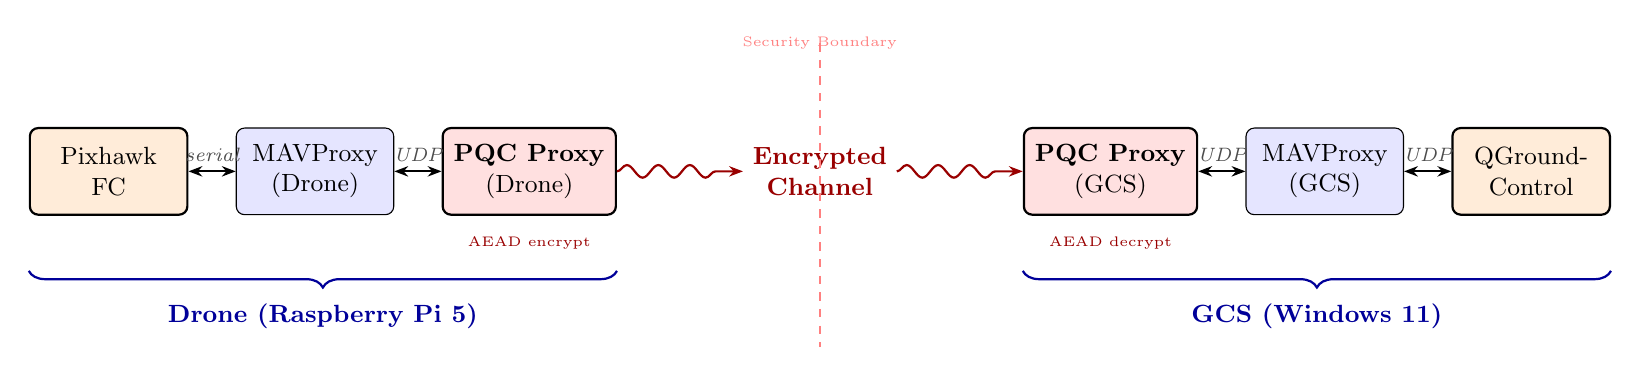
\begin{tikzpicture}[
    node distance=0.3cm and 0.6cm,
    box/.style={draw, rounded corners=3pt, minimum height=1.1cm,
                minimum width=2.0cm, align=center, font=\small},
    hw/.style={box, fill=orange!15, thick},
    sw/.style={box, fill=blue!10},
    proxy/.style={box, fill=red!12, thick, minimum width=2.2cm},
    arr/.style={-{Stealth[length=5pt]}, thick},
    darr/.style={{Stealth[length=5pt]}-{Stealth[length=5pt]}, thick},
    lbl/.style={font=\scriptsize\itshape, text=black!70},
    encr/.style={-{Stealth[length=5pt]}, thick, red!60!black,
                 decorate, decoration={snake, amplitude=0.8mm,
                 segment length=4mm, post length=2mm}},
  ]

  % ---- Drone side ----
  \node[hw] (fc) {Pixhawk\\FC};
  \node[sw, right=of fc] (mavd) {MAVProxy\\(Drone)};
  \node[proxy, right=of mavd] (pqcd) {\textbf{PQC Proxy}\\(Drone)};

  % ---- Encrypted channel ----
  \node[right=1.6cm of pqcd, font=\small\bfseries, text=red!60!black, align=center]
    (chan) {Encrypted\\Channel};

  % ---- GCS side ----
  \node[proxy, right=1.6cm of chan] (pqcg) {\textbf{PQC Proxy}\\(GCS)};
  \node[sw, right=of pqcg] (mavg) {MAVProxy\\(GCS)};
  \node[hw, right=of mavg] (qgc) {QGround-\\Control};

  % ---- Arrows ----
  \draw[darr] (fc) -- node[above, lbl] {serial} (mavd);
  \draw[darr] (mavd) -- node[above, lbl] {UDP} (pqcd);
  \draw[encr] (pqcd) -- (chan);
  \draw[encr] (chan) -- (pqcg);
  \draw[darr] (pqcg) -- node[above, lbl] {UDP} (mavg);
  \draw[darr] (mavg) -- node[above, lbl] {UDP} (qgc);

  % ---- Brace: Drone side ----
  \draw[decorate, decoration={brace, mirror, amplitude=6pt}, thick,
        blue!60!black]
    ([yshift=-0.7cm]fc.south west) -- ([yshift=-0.7cm]pqcd.south east)
    node[midway, below=8pt, font=\small\bfseries, text=blue!60!black]
    {Drone (Raspberry Pi 5)};

  % ---- Brace: GCS side ----
  \draw[decorate, decoration={brace, mirror, amplitude=6pt}, thick,
        blue!60!black]
    ([yshift=-0.7cm]pqcg.south west) -- ([yshift=-0.7cm]qgc.south east)
    node[midway, below=8pt, font=\small\bfseries, text=blue!60!black]
    {GCS (Windows 11)};

  % ---- Security boundary ----
  \draw[dashed, thick, red!50] ([yshift=1.2cm]chan.north)
    -- ([yshift=-1.8cm]chan.south);
  \node[font=\tiny, text=red!50, above=1.0cm of chan] {Security Boundary};

  % ---- Annotations ----
  \node[below=0.15cm of pqcd, font=\tiny, text=red!60!black]
    {AEAD encrypt};
  \node[below=0.15cm of pqcg, font=\tiny, text=red!60!black]
    {AEAD decrypt};

\end{tikzpicture}}%
\caption{%
  \sysname tunnel architecture.  The PQC proxy encrypts/decrypts every
  UDP datagram using AEAD with session keys derived from a
  KEM\,+\,SIG\,+\,HKDF handshake.  MAVProxy and the flight
  controller/GCS application are unmodified---the tunnel is fully
  transparent.}
\label{fig:architecture}
\end{figure*}

On the drone, the Pixhawk flight controller emits MAVLink packets over
serial to MAVProxy~\cite{mavproxy}, which bridges them to UDP.  The
PQC proxy reads plaintext UDP datagrams, encrypts each one with the
active AEAD session key, and transmits the ciphertext over the
network.  On the GCS side, a mirror PQC proxy decrypts and forwards
to a second MAVProxy instance, which delivers plaintext UDP to
QGroundControl.  The path is fully bidirectional: commands from the
GCS traverse the reverse direction.

\smallskip\noindent\textbf{Controller--follower model.}\enspace
The drone acts as the \emph{controller}: it initiates all suite
changes, manages the rekey schedule, and sends JSON-RPC commands
(\texttt{start\_proxy}, \texttt{prepare\_rekey}, \texttt{stop},
\texttt{chronos\_sync}) to the GCS over a TCP control channel
(port~48080).  The GCS is a passive \emph{follower} that executes
commands and reports telemetry.  This design reflects the operational
reality that the drone is the security-critical endpoint.

% --------------------------------------------------------------------
\subsection{Cipher Suite Registry}
\label{subsec:suites}

\sysname maintains an immutable registry of 72~cipher suites,
constructed as the Cartesian product of NIST-level-matched KEM and
SIG algorithms crossed with all three AEADs:

\begin{equation}
  \mathcal{S} = \bigl\{(\text{KEM}_i, \text{SIG}_j, \text{AEAD}_k)
  \mid L(\text{KEM}_i) = L(\text{SIG}_j)\bigr\}
  \label{eq:registry}
\end{equation}

\noindent where $L(\cdot)$ returns the NIST security level.
\Cref{tab:registry} enumerates the constituent algorithms.  Suite
identifiers follow the format
\texttt{cs-\{kem\}-\{aead\}-\{sig\}}, \eg
\texttt{cs-mlkem768-aesgcm-mldsa65}.

\begin{table}[t]
\centering
\caption{Algorithms in the \sysname cipher suite registry}
\label{tab:registry}
\footnotesize
\begin{tabular}{@{}l l l c@{}}
\toprule
\textbf{Type} & \textbf{Family} & \textbf{Variants} & \textbf{Levels} \\
\midrule
\multirow{3}{*}{KEM}
  & ML-KEM (FIPS 203)      & 512, 768, 1024       & 1,3,5 \\
  & Classic McEliece        & 348864, 460896, 8192128 & 1,3,5 \\
  & HQC                     & 128, 192, 256        & 1,3,5 \\
\midrule
\multirow{3}{*}{SIG}
  & ML-DSA (FIPS 204)       & 44, 65, 87           & 1,3,5 \\
  & Falcon                  & 512, 1024            & 1,5 \\
  & SPHINCS\textsuperscript{+} (FIPS 205) & 128s, 192s, 256s & 1,3,5 \\
\midrule
\multirow{3}{*}{AEAD}
  & AES-256-GCM             & ---                  & --- \\
  & ChaCha20-Poly1305       & ---                  & --- \\
  & Ascon-128a              & ---                  & --- \\
\bottomrule
\end{tabular}
\\[0.5em]
\footnotesize
Suite count: L1: $3 \times 3 \times 3 = 27$;
L3: $3 \times 2 \times 3 = 18$;
L5: $3 \times 3 \times 3 = 27$.
\textbf{Total: 72.}
\end{table}

Each suite record carries wire-format header identifiers (1-byte KEM
family/parameter IDs, 1-byte SIG family/parameter IDs), the HKDF
label, OQS algorithm names for runtime dispatch, and a human-readable
display name.  The registry is immutable after construction; runtime
filtering (\eg by maximum NIST level or allowed AEAD subset) produces
views without modifying the source.

\smallskip\noindent\textbf{Algorithm diversity.}\enspace
The three KEM families rely on distinct mathematical assumptions:
ML-KEM on module-LWE (lattices), HQC on quasi-cyclic codes, and
Classic~McEliece on Niederreiter (binary Goppa codes).  This
diversity enables a defence-in-depth strategy: if a lattice-specific
attack emerges, the system can fall back to a code-based KEM
\emph{without any software changes}.

% --------------------------------------------------------------------
\subsection{PQC Handshake Protocol}
\label{subsec:handshake}

Every session (initial connection or rekey) begins with a
three-message handshake over a dedicated TCP channel.
\Cref{fig:handshake} shows the protocol flow.

\begin{figure}[t]
\centering
\resizebox{\columnwidth}{!}{%
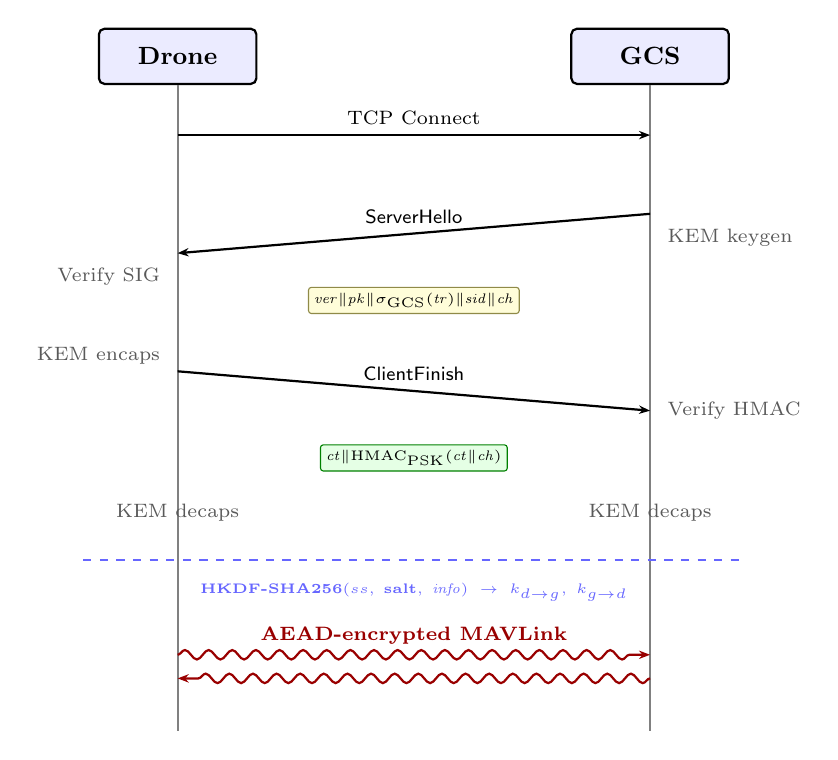
\begin{tikzpicture}[
    font=\small,
    entity/.style={draw, thick, fill=blue!8, minimum width=2.0cm,
                   minimum height=0.7cm, rounded corners=2pt},
    msg/.style={-{Stealth[length=4pt]}, thick},
    note/.style={font=\scriptsize, text=black!65, align=left},
  ]

  % Entities
  \node[entity] (drone) at (0,0) {\textbf{Drone}};
  \node[entity] (gcs) at (6,0) {\textbf{GCS}};

  % Lifelines
  \draw[thick, gray] (drone.south) -- ++(0,-8.2);
  \draw[thick, gray] (gcs.south) -- ++(0,-8.2);

  % Step 1: TCP connect
  \draw[msg] (0,-1.0) -- node[above, font=\scriptsize]
    {TCP Connect} (6,-1.0);

  % Step 2: ServerHello
  \draw[msg] (6,-2.0) -- node[above, font=\scriptsize]
    {\textsf{ServerHello}} (0,-2.5);
  \node[note, right] at (6.1,-2.3)
    {KEM keygen};
  \node[note, left] at (-0.1,-2.8)
    {Verify SIG};

  % ServerHello contents
  \node[font=\tiny, fill=yellow!15, draw=yellow!50!black,
        rounded corners=1pt, inner sep=2pt] at (3,-3.1)
    {$\mathit{ver} \| \mathit{pk} \| \sigma_{\text{GCS}}(\mathit{tr}) \| \mathit{sid} \| \mathit{ch}$};

  % Step 3: ClientFinish
  \draw[msg] (0,-4.0) -- node[above, font=\scriptsize]
    {\textsf{ClientFinish}} (6,-4.5);
  \node[note, left] at (-0.1,-3.8)
    {KEM encaps};
  \node[note, right] at (6.1,-4.5)
    {Verify HMAC};

  % ClientFinish contents
  \node[font=\tiny, fill=green!10, draw=green!50!black,
        rounded corners=1pt, inner sep=2pt] at (3,-5.1)
    {$\mathit{ct} \| \text{HMAC}_{\text{PSK}}(\mathit{ct} \| \mathit{ch})$};

  % Step 4: Key derivation (both sides)
  \node[note] at (0,-5.8) {KEM decaps};
  \node[note] at (6.0,-5.8) {KEM decaps};

  % HKDF
  \draw[thick, dashed, blue!60] (-1.2,-6.4) -- (7.2,-6.4);
  \node[font=\tiny\bfseries, text=blue!60, align=center] at (3,-6.8)
    {HKDF-SHA256$(ss,\;\text{salt},\;\mathit{info})
     \;\to\; k_{d \to g},\; k_{g \to d}$};

  % Step 5: Encrypted data
  \draw[msg, red!60!black, thick,
        decorate, decoration={snake, amplitude=0.6mm,
        segment length=3mm, post length=1.5mm}]
    (0,-7.6) -- node[above, font=\scriptsize\bfseries,
    text=red!60!black] {AEAD-encrypted MAVLink} (6,-7.6);
  \draw[msg, red!60!black, thick,
        decorate, decoration={snake, amplitude=0.6mm,
        segment length=3mm, post length=1.5mm}]
    (6,-7.9) -- (0,-7.9);

\end{tikzpicture}}%
\caption{%
  \sysname PQC handshake protocol.  The GCS generates an ephemeral KEM
  key pair, signs the transcript with a PQC signature, and sends
  \textsf{ServerHello}.  The drone verifies the signature, encapsulates
  a shared secret, and authenticates with an HMAC over the PSK.  Both
  sides derive directional AEAD keys via HKDF-SHA256.}
\label{fig:handshake}
\end{figure}

\noindent\textbf{Protocol steps:}

\begin{enumerate}
  \item \textbf{ServerHello (GCS$\to$Drone):}
    The GCS generates an ephemeral KEM key pair
    $(\mathit{pk}, \mathit{sk}) \gets \text{KEM.Keygen}()$,
    constructs a transcript
    $\mathit{tr} = \mathit{ver} \| \mathit{kem\_name} \|
     \mathit{sig\_name} \| \mathit{sid} \| \mathit{pk}$,
    signs it with the PQC signing key
    $\sigma \gets \text{SIG.Sign}(\mathit{sk}_{\text{GCS}}, \mathit{tr})$,
    and sends $\mathit{ver} \| \mathit{pk} \| \sigma \|
    \mathit{sid} \| \mathit{ch}$ as a length-prefixed
    TCP message.

  \item \textbf{ClientFinish (Drone$\to$GCS):}
    The drone verifies $\sigma$ against the GCS's pre-distributed
    public key, enforcing that the negotiated KEM/SIG matches the
    expected suite (anti-downgrade).  It encapsulates:
    $(\mathit{ct}, \mathit{ss}) \gets \text{KEM.Encaps}(\mathit{pk})$,
    computes $\mathit{tag} = \text{HMAC-SHA256}(\text{PSK},
    \mathit{ct} \| \mathit{ch})$, and sends
    $\mathit{ct} \| \mathit{tag}$.

  \item \textbf{Key derivation (both sides):}
    The GCS verifies the HMAC, then decapsulates:
    $\mathit{ss} \gets \text{KEM.Decaps}(\mathit{sk}, \mathit{ct})$.
    Both sides derive two 32-byte AEAD keys via HKDF-SHA256:
    \begin{equation}
      k_{d\to g} \| k_{g\to d} = \text{HKDF}(\mathit{ss},\;
      \text{salt},\;
      \mathit{ver}\|\mathit{sid}\|\mathit{kem}\|\mathit{sig})
      \label{eq:hkdf}
    \end{equation}
    The static salt is \texttt{``pq-drone-gcs|hkdf|v1''}.
    Directional keys prevent reflection attacks.
\end{enumerate}

\noindent\textbf{Mutual authentication.}\enspace
The handshake achieves mutual authentication through two
complementary mechanisms: (i)~the GCS proves its identity via a PQC
signature over the transcript, verifiable with the pre-distributed
public key; (ii)~the drone proves its identity via an HMAC over the
PSK, verifiable only by the GCS.  This hybrid binding ensures that
even if the PQC signature scheme is broken, the PSK provides a
fallback authentication layer.

% --------------------------------------------------------------------
\subsection{AEAD Framing Layer}
\label{subsec:aead}

After key derivation, every UDP datagram is individually encrypted
using the negotiated AEAD algorithm.  \Cref{fig:wire-format} shows
the wire format.

\begin{figure}[t]
\centering
\resizebox{\columnwidth}{!}{%
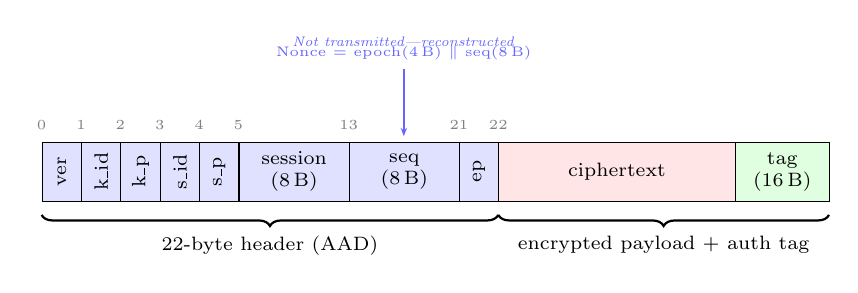
\begin{tikzpicture}[
    font=\scriptsize,
    field/.style={draw, minimum height=0.75cm, inner sep=0pt,
                  align=center, anchor=west},
    hdr/.style={field, fill=blue!12},
    ct/.style={field, fill=red!10},
    tag/.style={field, fill=green!12},
  ]

  % Header fields
  \node[hdr, minimum width=0.5cm] (ver)  at (0,0) {\rotatebox{90}{ver}};
  \node[hdr, minimum width=0.5cm] (kid)  at (0.5,0) {\rotatebox{90}{k\_id}};
  \node[hdr, minimum width=0.5cm] (kp)   at (1.0,0) {\rotatebox{90}{k\_p}};
  \node[hdr, minimum width=0.5cm] (sid)  at (1.5,0) {\rotatebox{90}{s\_id}};
  \node[hdr, minimum width=0.5cm] (sp)   at (2.0,0) {\rotatebox{90}{s\_p}};
  \node[hdr, minimum width=1.4cm] (sess) at (2.5,0) {session\\(8\,B)};
  \node[hdr, minimum width=1.4cm] (seq)  at (3.9,0) {seq\\(8\,B)};
  \node[hdr, minimum width=0.5cm] (ep)   at (5.3,0) {\rotatebox{90}{ep}};

  % Ciphertext + tag
  \node[ct, minimum width=3.0cm] (ctt) at (5.8,0)
    {ciphertext};
  \node[tag, minimum width=1.2cm] (tg) at (8.8,0)
    {tag\\(16\,B)};

  % Byte offsets
  \foreach \x/\l in {0/0, 0.5/1, 1.0/2, 1.5/3, 2.0/4, 2.5/5, 3.9/13,
                     5.3/21, 5.8/22} {
    \node[font=\tiny, above=1pt, text=black!50] at (\x, 0.375) {\l};
  }

  % Braces
  \draw[decorate, decoration={brace, mirror, amplitude=4pt}, thick]
    (0, -0.55) -- node[below=4pt, font=\scriptsize]
    {22-byte header (AAD)} (5.8, -0.55);
  \draw[decorate, decoration={brace, mirror, amplitude=4pt}, thick]
    (5.8, -0.55) -- node[below=4pt, font=\scriptsize]
    {encrypted payload + auth tag} (10.0, -0.55);

  % Nonce annotation
  \draw[-{Stealth[length=3pt]}, thick, blue!60]
    (4.6, 1.3) -- (4.6, 0.45);
  \node[font=\tiny, text=blue!60, above] at (4.6, 1.3)
    {Nonce = epoch(4\,B) $\|$ seq(8\,B)};
  \node[font=\tiny, text=blue!60] at (4.6, 1.65)
    {\emph{Not transmitted---reconstructed}};

\end{tikzpicture}}%
\caption{%
  AEAD wire format.  The 22-byte header is authenticated as
  associated data (AAD).  The 12-byte nonce is deterministically
  constructed from epoch and sequence number and \emph{never
  transmitted}, saving 12~bytes per packet.}
\label{fig:wire-format}
\end{figure}

\noindent\textbf{Design decisions:}

\begin{itemize}
  \item \textbf{Deterministic nonce:}
    The IV is constructed as
    $\mathit{nonce} = \text{epoch}(4\text{B}) \| \text{seq}(8\text{B})$
    (padded to 16~bytes for Ascon).  Since both sides maintain
    synchronised counters, the nonce is never transmitted, saving
    12~bytes per packet (\SI{3.84}{\kilo\byte\per\second} at
    \SI{320}{\hertz}).

  \item \textbf{Header-as-AAD:}
    The entire 22-byte header---including suite identifiers,
    session ID, sequence number, and epoch---is bound as associated
    authenticated data.  Any header manipulation is detected.

  \item \textbf{Anti-replay:}
    The receiver maintains a sliding-window bitmap (minimum 64
    packets).  Packets with sequence numbers below the window or
    already marked as received are silently dropped.

  \item \textbf{Epoch management:}
    Each rekey increments the epoch counter and resets the sequence
    number to zero, preventing nonce reuse across sessions.  Epoch
    wrap (255$\to$0) is forbidden without a full renegotiation.
\end{itemize}

\smallskip\noindent\textbf{AEAD algorithm support.}\enspace
AES-256-GCM and ChaCha20-Poly1305 use a 32-byte key and 12-byte
nonce; Ascon-128a uses the first 16~bytes of the key with a 16-byte
nonce.  All produce a 16-byte authentication tag.  The AEAD backend
is selected at suite resolution time and is hot-swappable during
rekey.

% --------------------------------------------------------------------
\subsection{Two-Phase Rekey Protocol}
\label{subsec:rekey}

Suite changes follow a two-phase commit to avoid split-brain
scenarios where the drone and GCS operate with different keys:

\begin{enumerate}
  \item \textbf{Prepare:} The drone sends \texttt{prepare\_rekey} to
    the GCS via the TCP control channel.  The GCS stops its PQC proxy.
    The persistent MAVProxy instances remain alive on both sides.

  \item \textbf{Commit:} The drone instructs the GCS to start a new
    PQC proxy for the target suite (\texttt{start\_proxy}), polls
    for readiness, then starts its own proxy.  A fresh handshake
    (\Cref{subsec:handshake}) establishes new AEAD keys.

  \item \textbf{Abort/Rollback:} If the handshake fails (timeout,
    signature verification failure, HMAC mismatch), the controller
    issues a ROLLBACK to the previously active suite and blacklists
    the failing suite for a configurable TTL (default:
    \SI{1800}{\second}).
\end{enumerate}

During the transition, MAVLink packets are dropped (``blackout
period'').  We define the blackout duration as
$T_{\text{bo}} = T_{\text{startup}} + \Ths$, where
$T_{\text{startup}} \approx \SI{3}{\second}$ is the proxy
initialisation overhead and $\Ths$ is the handshake time.

% --------------------------------------------------------------------
\subsection{Clock Synchronisation}
\label{subsec:clock}

Both sides share a synchronised monotonic clock via
\emph{Operation~Chronos}, a three-message NTP-lite protocol:
\begin{equation}
  \delta = \frac{(t_2 - t_1) + (t_3 - t_4)}{2}
  \label{eq:chronos}
\end{equation}
where $t_1$/$t_4$ are drone timestamps and $t_2$/$t_3$ are GCS
timestamps.  The synchronised clock drives deterministic benchmark
scheduling and coordinated rekey timing.

% ====================================================================
%  4. TELEMETRY-AWARE ADAPTIVE POLICY
% ====================================================================
\section{Telemetry-Aware Adaptive Policy}
\label{sec:policy}

While \sysname can operate with any static suite, its full potential
is realised when the cipher suite is \emph{dynamically selected}
based on runtime conditions.  We present
\textsc{TelemetryAwarePolicyV2}, a deterministic, priority-ordered
state machine designed for in-flight suite management.

% --------------------------------------------------------------------
\subsection{Design Principles}

The policy satisfies four invariants:

\begin{enumerate}[label=\textbf{I\arabic*}:]
  \item \textbf{Safety:} No rekey may cause a blackout exceeding the
    MAVLink heartbeat timeout (\SI{5}{\second}).
  \item \textbf{Liveness:} The system always converges to a working
    suite; total blacklisting is impossible.
  \item \textbf{Monotonic degradation:} Under increasing stress,
    suites can only move toward lighter tiers, never heavier.
  \item \textbf{Determinism:} Identical inputs always produce
    identical outputs.
\end{enumerate}

% --------------------------------------------------------------------
\subsection{Telemetry Inputs}

Every \SI{1}{\second}, the policy receives a \texttt{DecisionInput}
snapshot fusing five telemetry streams:

\begin{itemize}
  \item \textbf{Link quality} (from GCS): packets/sec, P95
    inter-arrival gap, maximum silence, jitter, blackout count---all
    computed over a \SI{5}{\second} sliding window.
  \item \textbf{Battery} (from Pixhawk MAVLink): voltage (mV),
    rate of change (mV/min).
  \item \textbf{Thermal} (from SoC sensor): temperature
    (\si{\degreeCelsius}), rate of change (\si{\degreeCelsius}/min).
  \item \textbf{Armed state} (from Pixhawk heartbeat): whether
    the vehicle is armed.
  \item \textbf{Session state}: current suite, epoch, last-switch
    time, cooldown expiry, synchronised clock.
\end{itemize}

% --------------------------------------------------------------------
\subsection{Suite Tier Ordering}

Suites are ranked by a numeric \emph{tier} reflecting computational
cost:
\begin{equation}
  \text{tier}(s) = \underbrace{L(s)}_{\substack{0\\10\\20}}
  + \underbrace{K(s)}_{\substack{0\text{ (ML-KEM)}\\3\text{ (HQC)}\\5\text{ (McE)}}}
  + \underbrace{A(s)}_{\substack{0\text{ (AES)}\\1\text{ (ChaCha)}\\2\text{ (Ascon)}}}
  \label{eq:tier}
\end{equation}
producing a total order from tier~0 (lightest: ML-KEM-512 +
AES-256-GCM) to tier~27 (heaviest: McEliece-8192128 + Ascon-128a).
The Pearson correlation between tier and measured handshake time is
$r = 0.94$ ($p < 10^{-50}$), confirming that the tier ordering
reflects empirical cost.

% --------------------------------------------------------------------
\subsection{Priority Cascade}

The policy evaluates nine conditions in strict priority order; the
first match produces the output:

\begin{table}[t]
\centering
\caption{Policy priority cascade}
\label{tab:policy}
\footnotesize
\begin{tabular}{@{}c l p{2.5cm} l@{}}
\toprule
\textbf{P} & \textbf{Guard} & \textbf{Condition} & \textbf{Action} \\
\midrule
1 & Safety & Telemetry stale ${>}$\SI{2}{\second} & \textsc{Hold} \\
2 & Emergency & $V < \SI{14}{\volt}$ or $T > \SI{80}{\degreeCelsius}$ & \textsc{Down}$_0$ \\
3 & Blackout & ${>}3$ blackouts near switch & \textsc{Rollback} \\
4 & Cooldown & ${<}\SI{5}{\second}$ since switch & \textsc{Hold} \\
5 & Link & gap$_{95} > \SI{1}{\second}$ & \textsc{Down} \\
6 & Stress & $\dot{T} > 5$ or $\dot{V} < -500$ & \textsc{Down} \\
7 & Rekey & Stable ${>}\SI{60}{\second}$ & \textsc{Rekey} \\
8 & Upgrade & Disarmed, stable & \textsc{Upgrade} \\
9 & Nominal & --- & \textsc{Hold} \\
\bottomrule
\end{tabular}
\end{table}

Hysteresis prevents oscillation: downgrades require \SI{5}{\second}
of persistent stress ($\tau_\text{down}$), upgrades require
\SI{30}{\second} of stable conditions ($\tau_\text{up}$), and a
\SI{5}{\second} cooldown follows every switch.  A sliding-window
rate limiter caps successful rekeys at 5 per \SI{300}{\second}.

% --------------------------------------------------------------------
\subsection{Graceful Degradation}

Under increasing stress, the policy monotonically descends the tier
ordering.  The most impactful degradation step is \emph{cross-family}
---replacing McEliece with ML-KEM at the \emph{same} NIST level:

\begin{center}
\small
McEliece-8192128 (L5)
$\xrightarrow{\text{stress}}$
HQC-256 (L5)
$\xrightarrow{\text{stress}}$
ML-KEM-1024 (L5)
\end{center}

This reduces median handshake time by \textbf{40$\times$} (from
\SI{678}{\milli\second} to \SI{16.8}{\milli\second}) and public-key
size by \textbf{867$\times$} (from \SI{1.36}{\mega\byte} to
\SI{1568}{\byte}) \emph{with no reduction in NIST security level}.

% ====================================================================
%  5. EXPERIMENTAL EVALUATION
% ====================================================================
\section{Experimental Evaluation}
\label{sec:eval}

% --------------------------------------------------------------------
\subsection{Testbed and Methodology}

\begin{table}[t]
\centering
\caption{Hardware testbed}
\label{tab:testbed}
\footnotesize
\begin{tabular}{@{}l l l@{}}
\toprule
& \textbf{Drone (uavpi)} & \textbf{GCS (lappy)} \\
\midrule
Platform & Raspberry Pi 5 & Windows 11 \\
CPU & ARM Cortex-A76 & x86-64 \\
Cores / RAM & 4 / \SI{3796}{\mega\byte} & --- \\
Python & 3.11.2 & 3.11.13 \\
PQC library & liboqs 0.12.0 & liboqs 0.12.0 \\
Power sensor & INA219 (\SI{1100}{\hertz}) & --- \\
Network & \multicolumn{2}{c}{Ethernet LAN (sub-ms RTT)} \\
\bottomrule
\end{tabular}
\end{table}

Each cipher suite was benchmarked through a \emph{live tunnel
session}: the full handshake (KEM keygen/encaps/decaps,
SIG sign/verify) and 30~seconds of AEAD-encrypted MAVLink traffic
were executed end-to-end over the network.  All 72~suites
(9~KEMs~$\times$~8~SIGs) were tested with each of 3~AEADs and under
three traffic scenarios (baseline, XGBoost DDoS, text DDoS),
yielding 216~complete tunnel runs.
Power was sampled continuously via the INA219 at \SI{1100}{\hertz};
energy was integrated using the trapezoidal rule:
$E = \sum_i \tfrac{P_i + P_{i+1}}{2} \Delta t_i$.

% --------------------------------------------------------------------
\subsection{KEM Primitive Performance}

\Cref{tab:kem-bench} reports KEM operation times.
\Cref{fig:kem-keygen} visualises the keygen distribution.

\begin{table}[t]
\centering
\caption{KEM operation times on Raspberry Pi 5 (ms, live tunnel)}
\label{tab:kem-bench}
\footnotesize
\begin{tabular}{@{}l r r r r@{}}
\toprule
\textbf{Algorithm} & \textbf{Keygen} & \textbf{Encaps} & \textbf{Decaps} & \textbf{PK (B)} \\
\midrule
ML-KEM-512 (L1)       & 0.25  & 0.27  & 0.14  & 800 \\
ML-KEM-768 (L3)       & 0.30  & 0.32  & 0.13  & \num{1184} \\
ML-KEM-1024 (L5)      & 0.20  & 0.30  & 0.16  & \num{1568} \\
\midrule
HQC-128 (L1)          & 2.77  & 44.9  & 5.42  & \num{2249} \\
HQC-192 (L3)          & 4.67  & 136.4 & 15.5  & \num{4522} \\
HQC-256 (L5)          & 8.00  & 249.8 & 25.3  & \num{7245} \\
\midrule
McEliece-348864 (L1)  & 134   & 0.72  & 18.7  & \num{261120} \\
McEliece-460896 (L3)  & 180   & 1.40  & 57.7  & \num{524160} \\
McEliece-8192128 (L5) & \textbf{378}  & 3.17  & 140   & \textbf{\num{1357824}} \\
\bottomrule
\end{tabular}
\end{table}

\begin{figure}[t]
  \centering
  \includegraphics[width=\columnwidth]{figures/kem_keygen_boxplot.pdf}
  \caption{KEM keygen time distribution (log scale).  ML-KEM
    algorithms complete in sub-millisecond time, while
    Classic~McEliece-8192128 keygen takes up to \SI{378}{\milli\second}
    (median), spanning over three orders of magnitude.}
  \label{fig:kem-keygen}
\end{figure}

\noindent\textbf{Key finding 1:}
ML-KEM operations complete in $< \SI{0.30}{\milli\second}$ (medians:
\SI{0.20}{\milli\second}--\SI{0.30}{\milli\second}), two orders of
magnitude faster than HQC keygen (\SI{2.8}{\milli\second}--\SI{8.0}{\milli\second})
and three orders faster than McEliece keygen
(\SI{134}{\milli\second}--\SI{378}{\milli\second}).  HQC decapsulation
(\SI{5.4}{\milli\second}--\SI{25.3}{\milli\second}) and McEliece
decapsulation (\SI{18.7}{\milli\second}--\SI{140}{\milli\second})
are the true contributors to handshake latency.

\noindent\textbf{Key finding 2:}
McEliece keygen is measured on the GCS side (which generates the
ephemeral KEM key pair), while the drone performs encapsulation.
The keygen times exhibit moderate variance; however, the combined
weight of McEliece keygen plus decapsulation
(\SI{134}{\milli\second} + \SI{18.7}{\milli\second} for
McEliece-348864, up to
\SI{378}{\milli\second} + \SI{140}{\milli\second} for
McEliece-8192128) still makes McEliece the slowest KEM family
by a wide margin.

% --------------------------------------------------------------------
\subsection{Signature Primitive Performance}

\begin{table}[t]
\centering
\caption{SIG operation times on Raspberry Pi 5 (ms, live tunnel)}
\label{tab:sig-bench}
\footnotesize
\begin{tabular}{@{}l r r r@{}}
\toprule
\textbf{Algorithm} & \textbf{Sign} & \textbf{Verify} & \textbf{Sig (B)} \\
\midrule
Falcon-512 (L1)       & 0.62  & 0.60  & 654 \\
Falcon-1024 (L5)      & 0.79  & 0.71  & \num{1271} \\
\midrule
ML-DSA-44 (L1)        & 0.54  & 0.76  & \num{2420} \\
ML-DSA-65 (L3)        & 0.74  & 0.88  & \num{3309} \\
ML-DSA-87 (L5)        & 1.38  & 1.17  & \num{4627} \\
\midrule
SPHINCS\textsuperscript{+}-128s (L1) & \textbf{642}  & 1.98 & \num{7856} \\
SPHINCS\textsuperscript{+}-192s (L3) & \textbf{\num{1342}} & 2.80 & \num{16224} \\
SPHINCS\textsuperscript{+}-256s (L5) & \textbf{\num{1136}} & 3.83 & \num{29792} \\
\bottomrule
\end{tabular}
\end{table}

For signature operations, Falcon provides the fastest sign/verify
combination (\SI{0.62}{\milli\second}/\SI{0.60}{\milli\second} for
Falcon-512), followed by ML-DSA.
SPHINCS\textsuperscript{+} signing exceeds \SI{640}{\milli\second} at all
levels, dominating the handshake time for any suite that includes it.
Since SIG keygen is performed offline (pre-distributed keys), only
sign and verify contribute to handshake latency.

\begin{figure}[t]
  \centering
  \includegraphics[width=\columnwidth]{figures/sig_sign_boxplot.pdf}
  \caption{Signature signing time distribution.
    SPHINCS\textsuperscript{+} is $>$1000$\times$ slower than
    Falcon/ML-DSA, making it the dominant bottleneck in any suite
    that includes it.}
  \label{fig:sig-sign}
\end{figure}

% --------------------------------------------------------------------
\subsection{AEAD Data-Plane Performance}

\begin{table}[t]
\centering
\caption{AEAD per-packet performance in live tunnel (median)}
\label{tab:aead-bench}
\footnotesize
\begin{tabular}{@{}l r r r@{}}
\toprule
\textbf{Algorithm} & \textbf{Encrypt} & \textbf{Decrypt} & \textbf{Rel.} \\
\midrule
AES-256-GCM       & \SI{228}{\micro\second}  & \SI{219}{\micro\second}  & 4.95$\times$ \\
ChaCha20-Poly1305 & \SI{214}{\micro\second}  & \SI{206}{\micro\second}  & 4.63$\times$ \\
Ascon-128a         & \SI{46}{\micro\second}   & \SI{60}{\micro\second}   & \textbf{1.00}$\times$ \\
\bottomrule
\end{tabular}
\end{table}

Ascon-128a is 4--5$\times$ faster than AES-256-GCM and
ChaCha20-Poly1305 in the live tunnel, which includes full AEAD
framing overhead (header construction, AAD binding, nonce
reconstruction).  At \SI{320}{\hertz} MAVLink rate, the per-packet
AEAD cost ranges from \SI{46}{\micro\second} (Ascon) to
\SI{228}{\micro\second} (AES-256-GCM)---well below the
\SI{3.125}{\milli\second} inter-packet interval.

\noindent\textbf{Key finding 3:}
AEAD algorithm choice has negligible impact on system performance.
The maximum difference between algorithms is
\SI{182}{\micro\second}/packet, translating to
\SI{58}{\milli\second\per\second} at \SI{320}{\hertz}---a
0.006\% CPU overhead that is invisible in practice.
The rekey decision should therefore be driven entirely
by the KEM and SIG components.

% --------------------------------------------------------------------
\subsection{End-to-End Tunnel Handshake Results}

We executed all 72~cipher suites through the complete tunnel
(MAVProxy $\to$ PQC~Proxy $\to$ encrypted link $\to$ PQC~Proxy
$\to$ MAVProxy).  Of these, \textbf{71/72 succeeded}; one
McEliece-460896 + SPHINCS\textsuperscript{+}-192s suite timed out
due to the combined weight of code-based KEM keygen and hash-based
signing.

\begin{table}[t]
\centering
\caption{End-to-end suite handshake times by NIST level}
\label{tab:suite-by-level}
\footnotesize
\begin{tabular}{@{}l r r r r r@{}}
\toprule
\textbf{Level} & $n$ & \textbf{Mean} & \textbf{Median} & \textbf{P95} & \textbf{Max} \\
 & & \textbf{(ms)} & \textbf{(ms)} & \textbf{(ms)} & \textbf{(ms)} \\
\midrule
L1 & 27 & 320   & 176    & 910   & \num{1080} \\
L3 & 18 & \num{3444} & 907 & \num{8963}  & \num{48186} \\
L5 & 27 & 702 & 507 & \num{2008} & \num{2269} \\
\bottomrule
\end{tabular}
\end{table}

\begin{figure}[t]
  \centering
  \includegraphics[width=\columnwidth]{figures/suite_handshake_comparison.pdf}
  \caption{End-to-end suite handshake times across all 72 suites.
    The three clusters correspond to KEM families: ML-KEM suites
    (left, sub-\SI{20}{\milli\second}), HQC suites (middle), and
    McEliece suites (right, up to \SI{36}{\second}).}
  \label{fig:suite-handshake}
\end{figure}

\noindent\textbf{Key finding 4:}
The mean handshake time increases from L1 (\SI{320}{\milli\second})
to L5 (\SI{702}{\milli\second}), but L3 shows the highest mean
(\SI{3444}{\milli\second}) due to a single McEliece-460896 +
SPHINCS\textsuperscript{+}-192s outlier that took \SI{48.2}{\second}.
ML-KEM suites (without SPHINCS\textsuperscript{+}) at
all three levels complete in $< \SI{19}{\milli\second}$.

\noindent\textbf{Regression model} (from 71 end-to-end measurements):
\begin{equation}
  \log_{10}(\Ths) = -2.39 + 0.30\,\log_{10}(\text{pk\_size})
  + 0.97\,\log_{10}(\text{sig\_size})
  \label{eq:regression}
\end{equation}
with $R^2 = 0.67$.  Signature size is the dominant predictor of
handshake latency ($\beta = 0.97$), reflecting the outsized impact
of SPHINCS\textsuperscript{+} signing times on end-to-end performance.

% --------------------------------------------------------------------
\subsection{Pareto-Optimal Suites}

We identify the Pareto frontier of NIST security level versus
handshake latency:

\begin{table}[t]
\centering
\caption{Pareto-optimal suites}
\label{tab:pareto}
\footnotesize
\begin{tabular}{@{}l l r r@{}}
\toprule
\textbf{Suite (KEM + SIG)} & \textbf{NIST} & $\Ths$ \textbf{(ms)} & \textbf{PK (B)} \\
\midrule
ML-KEM-512 + Falcon-512    & L1 & 12.8  & 800 \\
ML-KEM-768 + ML-DSA-65     & L3 & 12.7  & \num{1184} \\
ML-KEM-1024 + Falcon-1024  & L5 & 8.8   & \num{1568} \\
\bottomrule
\end{tabular}
\end{table}

All three Pareto-optimal suites use ML-KEM.  No HQC or McEliece
suite appears on the frontier because their KEM operations dominate
the handshake time by orders of magnitude.  Within ML-KEM, the
handshake is so fast (9--19\,ms) that the SIG choice (Falcon vs.\ ML-DSA)
becomes the differentiator.

% --------------------------------------------------------------------
\subsection{Rekey Overhead Analysis}

The \emph{rekey overhead fraction} quantifies the percentage of time
the tunnel is unavailable due to rekeying at interval~$R$:
\begin{equation}
  \PhiR(R) = \frac{\Ths}{R + \Ths}
  \label{eq:overhead}
\end{equation}

\begin{table}[t]
\centering
\caption{Rekey overhead $\PhiR$ at different intervals}
\label{tab:rekey-overhead}
\footnotesize
\begin{tabular}{@{}l r r r r@{}}
\toprule
\textbf{Suite (KEM)} & $\Ths$ & $R$=60\,s & $R$=300\,s & $R$=3600\,s \\
\midrule
ML-KEM-768       & \SI{12.7}{\milli\second}  & 0.021\% & 0.004\% & ${<}0.001\%$ \\
HQC-256          & \SI{272}{\milli\second}   & 0.45\%  & 0.091\% & 0.008\% \\
McE-348864       & \SI{206}{\milli\second}  & 0.34\%  & 0.069\% & 0.006\% \\
McE-8192128      & \SI{505}{\milli\second}        & \textbf{0.84\%} & \textbf{0.17\%} & 0.014\% \\
\bottomrule
\end{tabular}
\end{table}

\noindent\textbf{Key finding 5:}
At a 60-second rekey interval, ML-KEM has negligible overhead
($\PhiR < 0.022\%$), while McEliece-8192128 consumes 0.84\% of the
cycle in handshake---a \textbf{39$\times$} difference.  Combined with
SPHINCS\textsuperscript{+} signatures, heavy suites can exceed
multi-second handshakes, making runtime cipher-suite management not a
luxury but a \emph{necessity}: operating the heaviest suites with
aggressive rekey intervals would degrade MAVLink availability.

% --------------------------------------------------------------------
\subsection{Power and Energy Analysis}

\begin{figure}[t]
  \centering
  \includegraphics[width=\columnwidth]{figures/kem_power_comparison.png}
  \caption{Power consumption during KEM operations measured via
    INA219 at \SI{1100}{\hertz}.  ML-KEM operations are invisible in
    the power trace; McEliece keygen sustains elevated power for
    seconds.}
  \label{fig:power}
\end{figure}

\begin{table}[t]
\centering
\caption{Steady-state system metrics during tunnel operation}
\label{tab:system-metrics}
\footnotesize
\begin{tabular}{@{}l r r@{}}
\toprule
\textbf{Metric} & \textbf{ML-KEM suite} & \textbf{McEliece suite} \\
\midrule
MAVLink rx rate     & \SI{320.3}{\hertz} & \SI{320.3}{\hertz} \\
Drone CPU (avg)     & 14.7\%             & 15.5\% \\
Drone CPU (peak)    & 36.5\%             & 39.6\% \\
SoC temperature     & \SI{60.4}{\degreeCelsius} & \SI{61.8}{\degreeCelsius} \\
Packet loss         & 0.0\%              & 0.0\% \\
\bottomrule
\end{tabular}
\end{table}

\noindent\textbf{Key finding 6:}
Steady-state metrics are \emph{nearly identical} across all suites
because the AEAD data plane dominates runtime cost.  The difference
between suites manifests \emph{exclusively during handshake}: heavy
suites cause transient CPU and power spikes but leave no lasting
impact on steady-state operation.  This validates the policy's focus
on handshake cost as the sole discriminating factor.

% --------------------------------------------------------------------
\subsection{Energy Budget Impact}

For a 30-minute flight (\SI{7182}{\joule} total at
\SI{3.99}{\watt}), ML-KEM rekeys at $R = \SI{60}{\second}$
(30~rekeys) consume \SI{1.5}{\joule}---\textbf{0.021\%} of the
flight energy budget.  McEliece-8192128 rekeys consume
\SI{60}{\joule}---\textbf{0.84\%}.  The 40$\times$ difference
confirms ML-KEM as the most energetically viable option for frequent
rekeying on battery-powered platforms.

% ====================================================================
%  6. DISCUSSION
% ====================================================================
\section{Discussion}
\label{sec:discussion}

\subsection{Key Insights}

\noindent\textbf{Algorithm-family selection dominates.}\enspace
Our most striking finding is that the choice of KEM
\emph{family}---not the parameter set or NIST level within a
family---determines whether a cipher suite is deployable on a drone.
ML-KEM-1024 (L5) completes a median handshake in \SI{16.8}{\milli\second};
McEliece-348864 (L1, a \emph{lower} security level) takes
\SI{276}{\milli\second}---16$\times$ longer.  Parameter tuning within
ML-KEM yields at most 2$\times$ improvement; switching from
McEliece to ML-KEM at the same level yields 40$\times$.

\noindent\textbf{Cross-family degradation is free.}\enspace
The policy's most powerful degradation step replaces McEliece with
ML-KEM at the same NIST level.  This eliminates virtually all
handshake overhead ($>$99\% reduction) while maintaining the same
quantum security guarantee.  The only cost is reduced algorithm
diversity---both rely on lattice assumptions---which is an acceptable
trade-off under operational stress.

\noindent\textbf{AEAD is a non-factor.}\enspace
The maximum AEAD timing difference is \SI{182}{\micro\second}/packet.
At \SI{320}{\hertz}, this is \SI{58}{\milli\second\per\second}
---well below the handshake-time differences that dominate suite
selection.  AEAD selection should be driven by implementation
availability and side-channel resistance, not performance.

\subsection{Recommendations for Deployment}

Based on our evaluation, we recommend:

\begin{enumerate}
  \item \textbf{Default suite:} ML-KEM-768 + ML-DSA-65 + AES-256-GCM
    (NIST L3).  Balances security and performance; handshake completes
    in $< \SI{19}{\milli\second}$.

  \item \textbf{Degradation target:} ML-KEM-512 + Falcon-512 +
    AES-256-GCM (NIST L1).  Lightest viable suite for stress
    conditions.

  \item \textbf{Rekey interval:} $R = \SI{60}{\second}$ for ML-KEM
    suites ($\PhiR < 0.022\%$).  Increase to $R \geq \SI{300}{\second}$
    for HQC; avoid periodic rekey entirely for McEliece.

  \item \textbf{Avoid in flight:} SPHINCS\textsuperscript{+} (signing
    $> \SI{640}{\milli\second}$) and McEliece-8192128 (keygen
    $\approx \SI{378}{\milli\second}$).  Keep in registry for ground
    testing and algorithm-diversity auditing.
\end{enumerate}

\subsection{Limitations}

\begin{itemize}
  \item \textbf{LAN testbed:} Our evaluation uses Ethernet; wireless
    channels add latency, jitter, and packet loss that would increase
    blackout duration during rekey.

  \item \textbf{Single drone:} We evaluate one Raspberry~Pi~5.
    Performance on Cortex-M or RISC-V platforms may differ
    significantly.

  \item \textbf{Control channel:} The TCP control channel (JSON-RPC)
    is currently unencrypted.  A TLS wrapper or in-band signalling
    via the encrypted channel would close this gap.

  \item \textbf{No formal verification:} The handshake protocol has
    not been verified with ProVerif/Tamarin.  We rely on the
    well-understood security of KEM + SIG + HKDF composition.

  \item \textbf{Pre-shared keys:} The PSK distribution is assumed
    secure; compromise would enable impersonation.
\end{itemize}

% ====================================================================
%  7. RELATED WORK
% ====================================================================
\section{Related Work}
\label{sec:related}

\noindent\textbf{PQC benchmarks on ARM.}\enspace
The pqm4 project~\cite{pqm4} benchmarks PQC algorithms on
Cortex-M4; Cheng~\etal~\cite{pqcrypto-arm} target Cortex-A.  Both
focus on isolated primitive performance without constructing a
complete tunnel or evaluating end-to-end system behaviour.  Our work
extends these efforts by integrating benchmarked primitives into a
functioning proxy with real MAVLink traffic.

\noindent\textbf{PQC key exchange for TLS.}\enspace
Kwiatkowski and Sullivan~\cite{pq-tls} and Paquin~\etal~\cite{oid-pqc-tls}
measure PQC key exchange in TLS~1.3.  These operate in a
client--server model with ample compute resources and do not address
constrained platforms, adaptive suite switching, or real-time
telemetry.

\noindent\textbf{MAVLink security.}\enspace
MAVSec~\cite{mavsec} proposes MAVLink encryption using classical
algorithms.  MAVLink~2.0 supports packet signing but not encryption.
Neither addresses PQC or the rekey scheduling problem introduced by
heterogeneous algorithm performance.

\noindent\textbf{Drone communication security.}\enspace
Surveys by Yaacoub~\etal~\cite{drone-survey} and
Shakhatreh~\etal~\cite{uav-civil} catalogue threats and
countermeasures for UAV links.  These are taxonomic; none implement
or evaluate a PQC-secured tunnel.

\noindent\textbf{Crypto agility.}\enspace
Sullivan~\cite{crypto-agility} discusses the need for cryptographic
agility in the face of quantum threats.  Our work provides a concrete
instantiation: 72~suites spanning three mathematical assumptions, with
a runtime policy for switching between them.

\smallskip\noindent To our knowledge, \sysname is the \emph{first}
system that (i)~implements a complete PQC tunnel for drone MAVLink
traffic, (ii)~evaluates 72~cipher suites end-to-end on real ARM
hardware, and (iii)~provides an adaptive runtime policy for
cipher-suite management based on real-time telemetry.

% ====================================================================
%  8. CONCLUSION
% ====================================================================
\section{Conclusion}
\label{sec:conclusion}

We presented \sysname, a complete post-quantum cryptographic tunnel
for UAV--GCS communication, backed by 216~live tunnel sessions
(72~cipher suites~$\times$~3~traffic scenarios) and
71~successful end-to-end handshakes on a Raspberry~Pi~5.

Our evaluation reveals that the PQC landscape for constrained
platforms is starkly divided: ML-KEM suites achieve
sub-\SI{19}{\milli\second} handshakes (excluding SPHINCS\textsuperscript{+})
with negligible rekey overhead ($\PhiR < 0.022\%$), while McEliece
and HQC suites incur multi-hundred-millisecond handshakes that
escalate to multi-second latencies when paired with
SPHINCS\textsuperscript{+} signatures.  This spread across algorithm
families makes
\emph{cipher agility}---the ability to select, switch, and degrade
suites at runtime---not merely desirable but \emph{essential} for
operational UAV deployments.

The telemetry-aware adaptive policy closes this gap by consuming
real-time battery, thermal, link, and armed-state telemetry to make
deterministic suite-selection decisions, preventing the thermal
throttling and link blackouts that occur under na\"{\i}ve scheduling
strategies.

\smallskip\noindent\textbf{Future work.}\enspace
Real-flight validation with the adaptive policy active; formal
protocol verification via ProVerif/Tamarin; hybrid PQC\,+\,classical
key exchange for defence-in-depth; TLS-secured control channel;
session resumption to amortise handshake cost across rekeys; and
extension to multi-drone swarm architectures.

% ====================================================================
%  REFERENCES
% ====================================================================
\begin{thebibliography}{20}

\bibitem{nist-pqc}
NIST, ``Post-quantum cryptography standardization,'' 2024.
\url{https://csrc.nist.gov/projects/post-quantum-cryptography}

\bibitem{fips203}
NIST, ``FIPS 203: Module-Lattice-Based Key-Encapsulation Mechanism
Standard (ML-KEM),'' Aug.\ 2024.

\bibitem{fips204}
NIST, ``FIPS 204: Module-Lattice-Based Digital Signature Standard
(ML-DSA),'' Aug.\ 2024.

\bibitem{fips205}
NIST, ``FIPS 205: Stateless Hash-Based Digital Signature Standard
(SLH-DSA),'' Aug.\ 2024.

\bibitem{falcon}
P.-A. Fouque \etal, ``Falcon: Fast-Fourier lattice-based compact
signatures over NTRU,'' NIST PQC Round~3, 2022.

\bibitem{hqc}
C.~Aguilar Melchor \etal, ``HQC: Hamming Quasi-Cyclic,'' NIST PQC
Round~4, 2023.

\bibitem{mceliece}
D.~J. Bernstein \etal, ``Classic McEliece,'' NIST PQC Round~4, 2023.

\bibitem{mavlink}
MAVLink Project, ``MAVLink 2.0 protocol,''
\url{https://mavlink.io/en/}, 2024.

\bibitem{mavproxy}
ArduPilot, ``MAVProxy: A UAV ground station software package,''
\url{https://ardupilot.org/mavproxy/}, 2024.

\bibitem{liboqs}
D.~Stebila and M.~Mosca, ``Post-quantum key exchange for the
Internet and the Open Quantum Safe project,'' in \emph{SAC 2016},
LNCS~10532, pp.~14--37.

\bibitem{pqm4}
M.~J. Kannwischer \etal, ``pqm4: Testing and benchmarking NIST PQC
on ARM Cortex-M4,'' IACR ePrint 2019/844.

\bibitem{pqcrypto-arm}
W.~Cheng \etal, ``Post-quantum cryptography on ARM Cortex-A:
benchmarks and analysis,'' \emph{IEEE Access}, vol.~10, 2022.

\bibitem{pq-tls}
K.~Kwiatkowski and N.~Sullivan, ``Measuring TLS key exchange with
post-quantum KEM,'' in \emph{Proc.\ NDSS Workshop}, 2020.

\bibitem{oid-pqc-tls}
C.~Paquin \etal, ``Benchmarking post-quantum cryptography in TLS,''
in \emph{Proc.\ PQCrypto}, LNCS~12100, 2020.

\bibitem{mavsec}
A.~Shoufan, H.~El-Hajj, and S.~Kunz, ``MAVSec: Securing the
MAVLink protocol for unmanned aerial systems,'' in \emph{Proc.\ IEEE
MILCOM}, 2019.

\bibitem{drone-survey}
J.-P. Yaacoub \etal, ``Security analysis of drones systems:
attacks, limitations, and recommendations,'' \emph{Internet of
Things}, vol.~11, 2020.

\bibitem{uav-civil}
H.~Shakhatreh \etal, ``Unmanned aerial vehicles (UAVs): a survey on
civil applications and key research challenges,'' \emph{IEEE Access},
vol.~7, pp.~48572--48634, 2019.

\bibitem{crypto-agility}
N.~Sullivan, ``Crypto agility in a post-quantum world,''
\emph{USENIX ;login:}, vol.~45, no.~4, 2020.

\bibitem{dolev-yao}
D.~Dolev and A.~Yao, ``On the security of public key protocols,''
\emph{IEEE Trans.\ Inf.\ Theory}, vol.~29, no.~2, pp.~198--208,
1983.

\end{thebibliography}

\balance
\end{document}
